\documentclass{beamer}

\usepackage{pri}
% \usepackage{breakurl}

\graphicspath{{./}{figures/}{figures/01-apresentacao/}}

\title{Processamento e Recuperação de Informação}

\subtitle{Apresentação da Disciplina}

\begin{document}

\maketitle

\begin{frame} 
    \frametitle{Apresentação}
    \begin{block}{Professores}
        \begin{itemize}
        \item Bruno Martins (responsável)
        \item Pável Calado
        \end{itemize}
    \end{block}
    \begin{block}{Tema da Disciplina}
        Busca, extração e análise de informação expressa \emph{textualmente}, e.g. existente na World Wide Web.
    \end{block}
    \begin{block}{Aulas}
        \begin{itemize}
        \item Teóricas: Conceitos Fundamentais + Teoria + Exemplos
        \item Laboratório: Problemas Práticos + Exercícios
        \end{itemize}
    \end{block}
    \small\hfill (horário de atendimento no Fénix) 
\end{frame}

\begin{frame} \frametitle{O que vão aprender...}
    \begin{itemize}
	\item Projetar soluções modernas para o processamento, gestão e interrogação de grandes volumes de informação não estruturada ou semi-estruturada;
	\item Classificar e agrupar automaticamente conjuntos de recursos (e.g., grandes conjuntos de documentos de texto) através de características descritivas;
	\item Conceber sistemas para a recuperação e filtragem da informação relevante existente em grandes coleções, com base em termos chave, com base em exemplos, ou com base em perfis dos utilizadores;
	\item Conceber sistemas para a extração de informação desde documentos de texto, ou desde a Web;
	\item Avaliar comparativamente diferentes sistemas para a extração, filtragem e recuperação de informação relevante.	
    \end{itemize}
\end{frame}

\begin{frame}
    \frametitle{Material de Apoio}
    \begin{block}{Bibliografia Principal}
        \scriptsize 
        Ricardo Baeza-Yates and Berthier Ribeiro-Neto, \textbf{Modern Information Retrieval}, 2ª ed. (2011)\\
        {\tiny\url{http://www.mir2ed.org}}\\[.5\baselineskip]

        Bing Liu, \textbf{Web Data Mining}, 2ª ed. (2011)\\
        {\tiny\url{http://www.cs.uic.edu/~liub/WebMiningBook.html}}
    \end{block}
    \begin{block}{Bibliografia Secundária}
        \scriptsize 
        Christopher D.  Manning, Prabhakar Raghavan and Hinrich Schütze,
        \textbf{Introduction to Information Retrieval} (2008)\\
        {\tiny\url{http://nlp.stanford.edu/IR-book/}}\\[.5\baselineskip]

        Anand Rajaraman, Jure Leskovec and Jeffrey D. Ullman, \textbf{Mining of Massive Datasets} (2013)\\
        {\tiny\url{http://infolab.stanford.edu/~ullman/mmds.html}}\\[.5\baselineskip]

        Ian H. Witten, Alistair Moffat, Timothy C. Bell, \textbf{Managing Gigabytes: Compressing and Indexing Documents and Images}, 2ª ed. (2000)\\
        {\tiny\url{http://people.eng.unimelb.edu.au/ammoffat/mg/}}
    \end{block}
    Outras referências serão disponibilizadas ao longo do semestre.
\end{frame}

\begin{frame} 
    \frametitle{Avaliação}
    \begin{itemize}
    \item Exame (individual) = 60\%; nota mínima = 9.5
%    \item Exercícios semanais (grupo) = 10\%
    \item Projeto(s) (grupo) = 40\%; nota mínima = 9.5
    \item Penalização para diferenças grandes entre notas de projetos exames:
    
    \begin{itemize}
    \item Se a nota $p$ dos projetos for superior à nota $e$ do exame em mais de 2 valores, a nota final $n$ será calculada com base na formula $n = x * e + (1-x) * p$, em que $x = 0.5 + \frac{|p-e|}{20}$.
    \end{itemize}
    
    \item Poderemos solicitar apresentação do(s) projeto(s)
    \end{itemize}
    
    ~\\
    
    Grupos de \emph{3 alunos}. As inscrições serão anunciadas em breve.
    
    ~\\
    
    Exame com consulta, mas limitada a \emph{uma folha A4 manuscrita}.
    
\end{frame}

\begin{frame}
  \frametitle{Ainda Sobre a Avaliação}
  \begin{block}{}
  Uma boa nota da disciplina implica {{\bf simultaneamente uma boa nota no projeto e no exame}.
  ~\\~\\
  Por exemplo:
  
 \begin{itemize}
 \item 18 no projeto e 10 no exame = 11 valores (e não 15)
 \item 17 no projeto e 12 no exame = 13 valores
 \end{itemize}
  }.
  \end{block}
  \begin{center}
    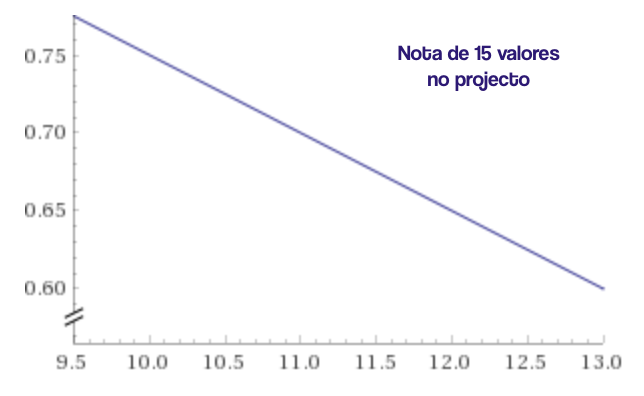
\includegraphics[width=0.45\textwidth]{15.png} ~~~~~~~
    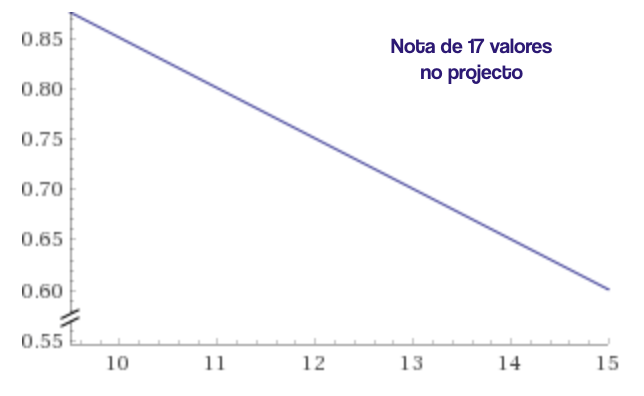
\includegraphics[width=0.45\textwidth]{17.png}
  \end{center}
\end{frame}


\begin{frame} 
    \frametitle{Trabalhadores-Estudantes e Época Especial} 
   \begin{block}{Avaliação para Trabalhadores-Estudantes}
   \begin{itemize}
    \item Mesmo método de avaliação;
	\item Alternativamente, alunos podem optar por método de avaliação com apenas um componente, i.e. o exame.
   \end{itemize}
   Quem fizer projeto em grupo será avaliado como aluno regular
   \end{block}
   \begin{block}{Avaliação em Época Especial}
   \begin{itemize}
   \item Avaliação com base num exame.
   \end{itemize}
   \end{block}
\end{frame}

\begin{frame} 
    \frametitle{Datas para Avaliação}
    \begin{itemize}
	\item Projeto 1 : Entrega a 03/11/2017 
	\item Projeto 2 : Entrega a 07/12/2017
    \item Exame 1 : 11/01/2018 - 11h30
    \item Exame 2 : 03/02/2018 - 09h00
    \end{itemize}
\end{frame}


\begin{frame} 
    \frametitle{Programa}
    \begin{enumerate}
    \footnotesize
	\item Introdução à extração e recuperação de informação 
%	◦	Arquitetura geral de sistemas de IR/IE 
%	◦	Pré-processamento de documentos em IR/IE 
	\item Modelos para dados não estruturados 
%	◦	O modelo booleano para recuperação de informação (RI) 
%	◦	Pesagem de termos e o modelo do espaço vectorial 
%	◦	Redução de dimensionalidade e latent semantic indexing 
%	◦	Modelos probabilísticos, o modelo BM25, e modelos de linguagem para RI 
	\item Informação não estruturada e extração de informação desde texto 
%	◦ Classificação e agrupamento automático de documentos 
%	◦	Classificação de documentos com o modelo naive Bayes 
%	◦	Extracção de informação com hidden Markov models 
	\item Avaliação em recuperação e extração de informação 
%	◦	Métricas de avaliação (precisão, abrangência, MAP, NDCG) 
%	◦	Coleções de referência, o TREC e a metodologia de avaliação de Cranfield 
%	◦	validação cruzada e outras considerações práticas 
	\item Modelos para dados semi-estruturados 
%	◦	Modelos de dados semi-estruturados (e.g., baseados em JSON) 
%	◦	A Extensible Markup Language (XML) e tecnologias relacionadas (e.g., XPath) 
%	◦	Linguagens de markup baseadas em XML (e.g., TEI, METS, MODS) 
%	◦	Outros modelos e linguagens de markup (e.g., SGML, HTML e RDF) 
	\item Informação semi-estruturada e extração de dados da Web 
%	◦	Geração de wrappers e extração de informação a partir de recursos na Web 
%	◦	Consultas a dados semi-estruturados e a linguagem XQuery 
%	◦	Recuperação de informação em coleções de dados XML 
	\item Análise de hiperligações e recuperação de informação na Web 
%	◦	Modelos da Web 
%	◦	Conceitos gerais sobre grafos e métodos de análise de hiperligações 
%	◦ Ordenação de resultados em motores de busca na Web, com base na análise de hiperligações 
%	◦	Recolha de dados da Web 
	\item Indexação e consulta de informação não estruturada
%	◦	Expressões regulares 
%	◦	Índices invertidos e construção eficiente de índices 
%	◦ Processamento de consultas com índices invertidos 
	\item Pesquisa por similaridade em dados multi-dimensionais 
%	◦	Shingling de documentos e a medida de similaridade de Jaccard entre conjuntos de documentos 
%	◦	Similarity-preserving sumaries of sets e a técnica min-hash 
%	◦	Locality-sensitive hashing 
%	◦	Aplicações em recuperação de informação multimédia 
	\item Sistemas de recomendação 
%	◦	Contexto, personalização, e filtragem de informação 
%	◦	Sistemas de recomendação com base no conteúdo 
%	◦	Sistemas de filtragem colaborativa 
	\item Técnicas de processamento distribuído para IR e IE 
%	◦	Particionamento de dados e técnicas distribuídas para IR/IE 
%	◦	Consultas federadas e sistemas de meta-pesquisa 
%	◦	Processamento map-reduce na gestão de dados da Web 
	\item {\it Aplicações para as técnicas de IE e IR}
%	◦	Enterprise search e pesquisa de peritos 
%	◦	Bibliotecas digitais 
%	◦	Prospecção de opiniões em conteúdos online 
%	◦	Outras aplicações (e.g., publicidade online)
	\end{enumerate}
\end{frame}

\begin{frame}
    \frametitle{Laboratórios e Implementação}
    \begin{center}
        Linguagem de programação: \textbf{Python} \\[.5\baselineskip]
    \end{center}
    \begin{block}{Recomendações:}
        \begin{itemize}
        \item Comecem a praticar \emph{hoje!}
        \item Formem os grupos \emph{o mais depressa possível}
        \item Usem os vossos portáteis nas aulas de lab., se possível
        \end{itemize}
    \end{block}
\end{frame}

\begin{frame}
    \frametitle{Python}    
    \begin{block}{Para começar:}
        \footnotesize
        \begin{description}
        \item[Python Programming Language] \url{http://www.python.org/}
        \item[The Python Tutorial] \url{http://docs.python.org/tutorial/}
        \item[Dive Into Python] \url{http://www.diveintopython.net/}
        \item[The Python Standard Library] \url{http://docs.python.org/library/}
        \end{description}
    \end{block}
    \begin{block}{Outras ferramentas úteis:}
        \footnotesize
        \begin{description}
        \item[Natural Language Toolkit] \url{http://nltk.org/}
        \item[Whoosh] \url{http://pypi.python.org/pypi/Whoosh/}
        \item[Beautiful Soup] \url{http://www.crummy.com/software/BeautifulSoup/}
        \item[feedparser] \url{http://code.google.com/p/feedparser/}
        \item[NumPy] \url{http://www.numpy.org/}
        \item[scikit-learn] \url{http://scikit-learn.org/}
        \item ... e outras a ser apresentadas ao longo das aulas
        \end{description}
    \end{block}
\end{frame}

\begin{frame}
    \begin{block}{}
        \centering
        \Large
        Mais questões?
    \end{block}
\end{frame}


\end{document}